\section{U-Net++}
\label{sec:Chapter23}

Architektura U-Net++ byla představena v roce 2018 v literatuře \cite{unetpp} jako vylepšení původní CNN architektury U-Net. Hypotézou této CNN architektury je zlepšení zachycení informací získaných v části enkodéru a následné obohacení o informace z hlubokých konvolučních bloků nahrazující plané skokové propojení původní sítě U-Net. Tyto obohacující konvoluční bloky byly přidány jako vyplnění sémantické trhliny ve skokových propojeních mezi enkodérem a dekodérem původní sítě U-Net. Přijímají také vstup ze všech předchozích bloků na stejné úrovni a výstup bloku z nižší vrstvy, na kterou je aplikována $2\times2$ vrstva typu up-sampling nebo transpose. Podoba sítě U-Net++ může být vyobrazena na obrázku \ref{fig:unetpp} v části a):

\begin{figure}[H]
\centering
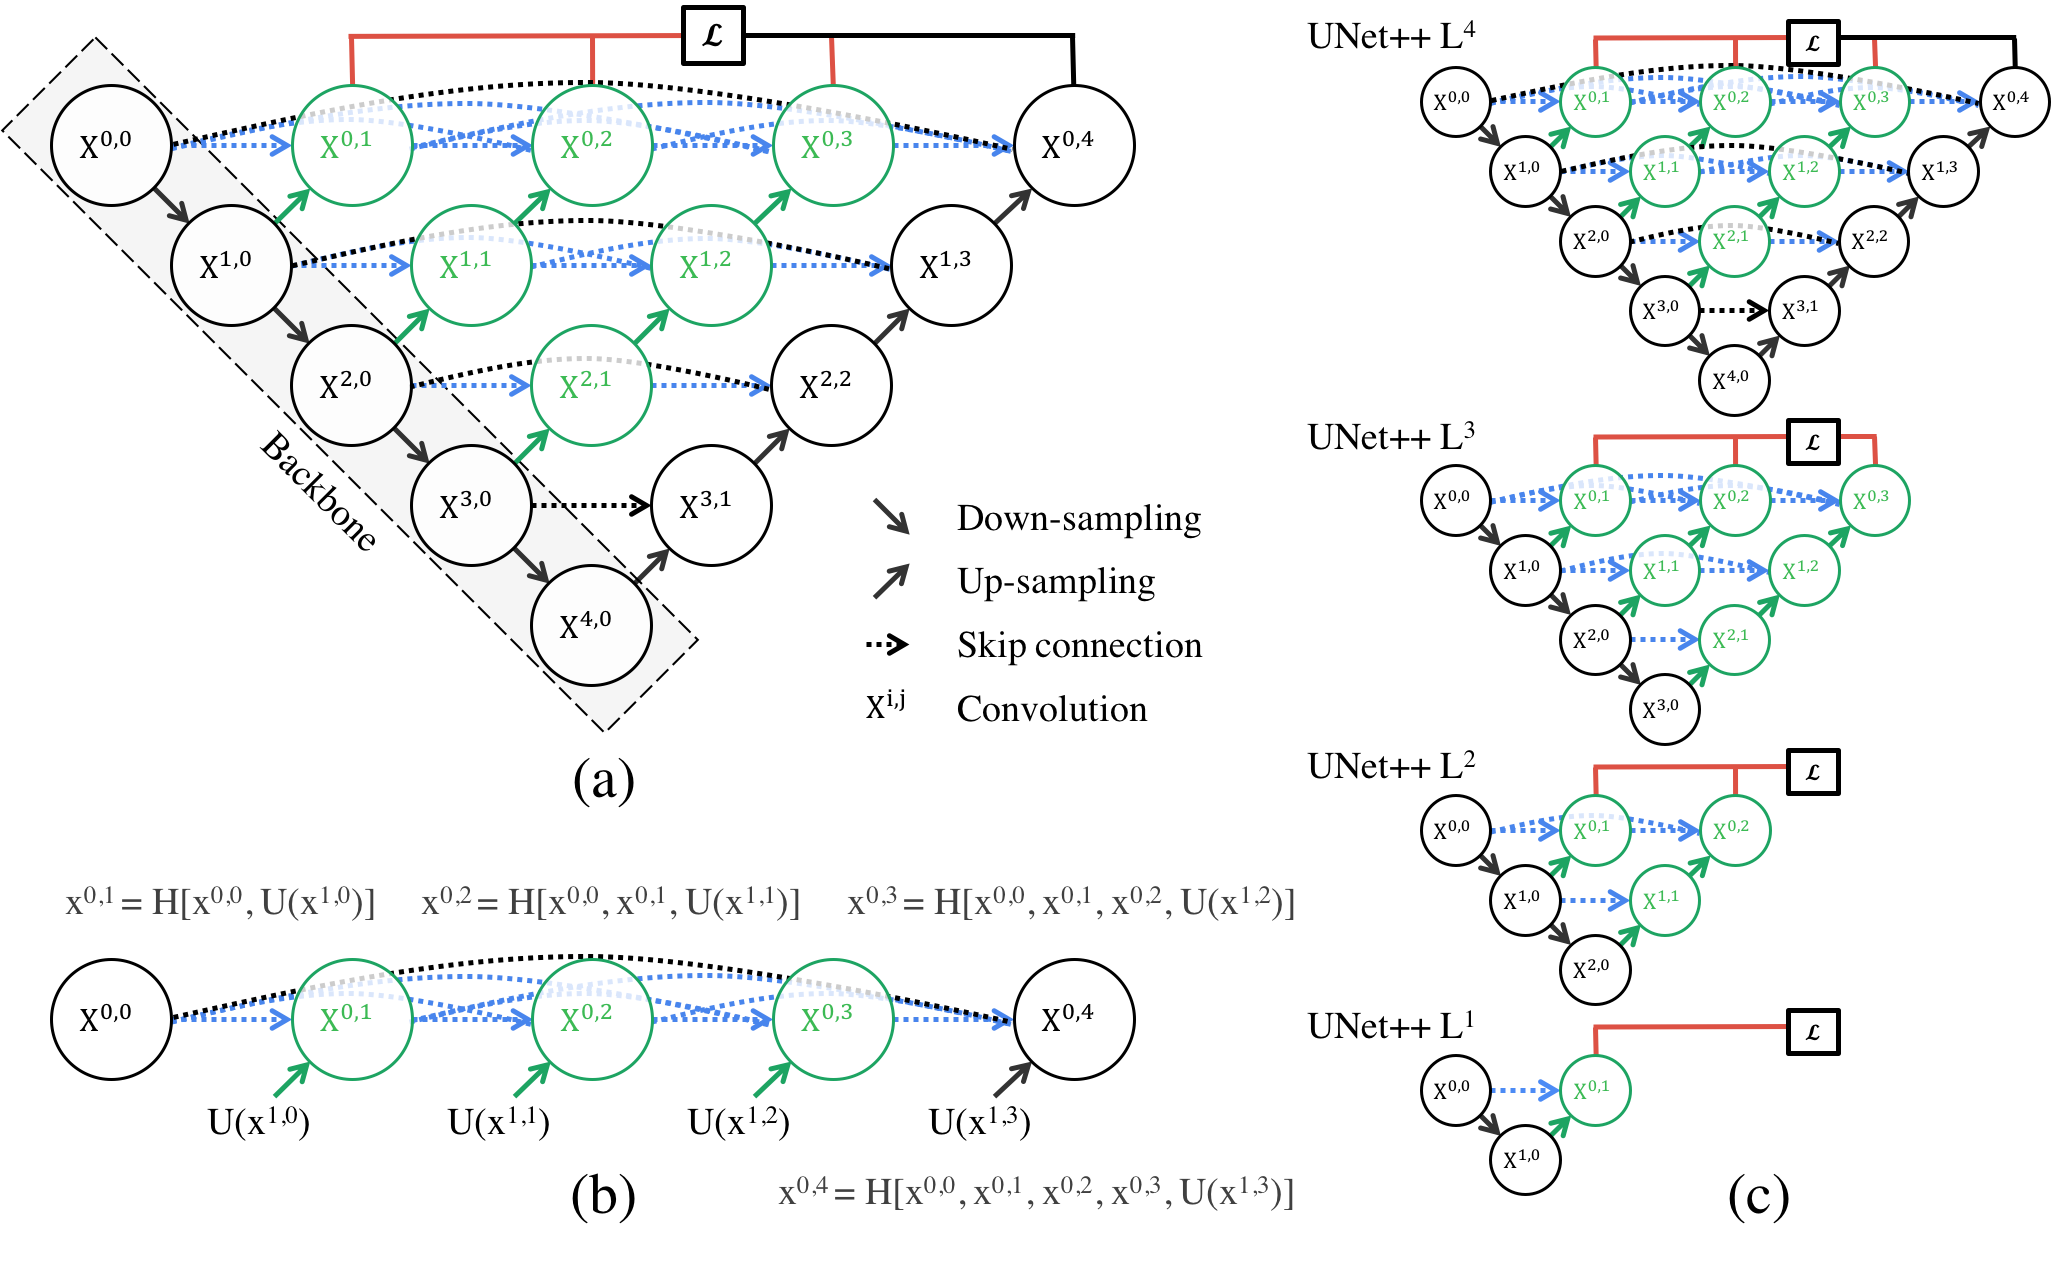
\includegraphics[width=1.0\textwidth,keepaspectratio]{Figures/unetpp.png}
\caption[Architektura sítě U-Net++]
{Architektura sítě U-Net++, kde je a) obecný pohled na síť architektury U-Net++ s přidanými skokovými bloky a hlubokou supervizí \uppercase\expandafter{\romannumeral 50 \relax} b) vrchní vrstva sítě U-Net mezi enkodérem a dekodérem, obsahující skokové bloky a jejich relevantní předcházející spoje c) různé možnosti rychlého režimu modelu díky hluboké supervizi. Převzato z \cite{unetpp}. }
\label{fig:unetpp}
\end{figure}

U-Net++ představuje i druhou změnu -- možnost \textbf{hluboké supervize}. Pokud byla síť trénována v módu hluboké supervize, pak hluboká supervize nám dovoluje využívat model při inferenci v jednom ze dvou režimů:

\begin{enumerate}
    \item \textbf{Přesný režim}, kde se využívají všechny bloky v blocích \{\(x^{0, j} \colon j \in \{1,2,...,n\}\)\}, kde \(n\) tvoří počet bloků v první (nejméně hluboké) vrstvě konvolučních bloků propojující enkodér-dekodér sítě U-Net++ \cite{unetpp}. V tomto režimu využíváme všechny pomocné výstupy těchto bloků, kde výstupní mapa příznaků tvoří průměr map příznaků těchto výstupů.
    \item \textbf{Rychlý režim}, kde použijeme tzv. pruning (vyobrazen na obrázku \ref{fig:unetpp} v části c) pro snížení velikosti (a tedy i parametrů) sítě, kde výslednou mapu tvoří poslední konvoluční blok v první vrstvě mezibloků sítě U-Net++. Síť v tomto režimu dokáže pracovat rychleji, zato méně přesněji.
\end{enumerate}

Při použití sítě U-Net++ v režimu hluboké supervize avšak výběr účastnících se bloků na finální mapě příznaků záleží na finální volbě implementace. Samozřejmě pro každý použití výstup se aplikuje relevantní výstupní vrstva, např. $1\times1\times1$ konvoluční vrstva s aktivační funkci sigmoid.

\endinput